\documentclass[12pt,letterpaper]{article}
\usepackage{graphicx,textcomp}
\usepackage{natbib}
\usepackage{setspace}
\usepackage{fullpage}
\usepackage{color}
\usepackage[reqno]{amsmath}
\usepackage{amsthm}
\usepackage{fancyvrb}
\usepackage{amssymb,enumerate}
\usepackage[all]{xy}
\usepackage{endnotes}
\usepackage{lscape}
\newtheorem{com}{Comment}
\usepackage{float}
\usepackage{hyperref}
\newtheorem{lem} {Lemma}
\newtheorem{prop}{Proposition}
\newtheorem{thm}{Theorem}
\newtheorem{defn}{Definition}
\newtheorem{cor}{Corollary}
\newtheorem{obs}{Observation}
\usepackage[compact]{titlesec}
\usepackage{dcolumn}
\usepackage{tikz}
\usetikzlibrary{arrows}
\usepackage{multirow}
\usepackage{subcaption}
\usepackage{xcolor}
\newcolumntype{.}{D{.}{.}{-1}}
\newcolumntype{d}[1]{D{.}{.}{#1}}
\definecolor{light-gray}{gray}{0.65}
\usepackage{url}
\usepackage{listings}
\usepackage{color}

\definecolor{codegreen}{rgb}{0,0.6,0}
\definecolor{codegray}{rgb}{0.5,0.5,0.5}
\definecolor{codepurple}{rgb}{0.58,0,0.82}
\definecolor{backcolour}{rgb}{0.95,0.95,0.92}

\lstdefinestyle{mystyle}{
	backgroundcolor=\color{backcolour},   
	commentstyle=\color{codegreen},
	keywordstyle=\color{magenta},
	numberstyle=\tiny\color{codegray},
	stringstyle=\color{codepurple},
	basicstyle=\footnotesize,
	breakatwhitespace=false,         
	breaklines=true,                 
	captionpos=b,                    
	keepspaces=true,                 
	numbers=left,                    
	numbersep=5pt,                  
	showspaces=false,                
	showstringspaces=false,
	showtabs=false,                  
	tabsize=2
}
\lstset{style=mystyle}
\newcommand{\Sref}[1]{Section~\ref{#1}}

\title{PS1 Response 19336078}
\date{26/06/2024}
\author{Owen Eglinton}

\begin{document}
\maketitle

\vspace{.25cm}

My first step was to set the working directory:

\lstinputlisting[language=R, firstline=32, lastline=32]{PS01_19336078.R}

\vspace{.25cm}

\section*{Question 1}

\vspace{.25cm}

I began by loading in the data:

\lstinputlisting[language=R, firstline=38, lastline=38]{PS01_19336078.R}  

\vspace{.25cm}

\begin{enumerate} 
	\item Find a 90\% confidence interval for the average student IQ in the school.
\end{enumerate}

I coded the process of finding the necessary descriptive statistics and using them to calculate the upper and lower bounds of the CI as follows: 

\lstinputlisting[language=R, firstline=42, lastline=47]{PS01_19336078.R}  

After running this code, I got the following output:

\begin{verbatim}
	[1] "The 90% CI for average student IQ is 93.96 - 102.92"
\end{verbatim}

\vspace{.25cm}

\begin{enumerate}
	\setcounter{enumi} 1
	\item Next, the school counselor was curious  whether  the average student IQ in her school is higher than the average IQ score (100) among all the schools in the country. Using the same sample, conduct the appropriate hypothesis test with $\alpha=0.05$.
\end{enumerate}

I set up a one-tailed t-test as follows: 

\lstinputlisting[language=R, firstline=51, lastline=51]{PS01_19336078.R}  

\noindent and got the following output:

\begin{verbatim}
	One Sample t-test

	data:  y
	t = -0.59574, df = 24, p-value = 0.7215
	alternative hypothesis: true mean is greater than 100
	95 percent confidence interval:
	93.95993      Inf
	sample estimates:
	mean of x 
	98.44 
\end{verbatim}

Since the \texttt{p-value} is greater than $\alpha$, we fail to reject the null hypothesis, and thus must conclude that the average student IQ is not greater than 100.

\vspace{.5cm}

\section*{Question 2}

\vspace{.25cm}

I began by loading in the data:

\lstinputlisting[language=R, firstline=57, lastline=57]{PS01_19336078.R}  

\vspace{.5cm}

\begin{enumerate} 
	\item Please plot the relationships among \emph{Y}, \emph{X1}, \emph{X2}, and \emph{X3}? What are the correlations among them (you just need to describe the graph and the relationships among them)?
\end{enumerate}

First, I imported the data descriptions as a label vector:

\lstinputlisting[language=R, firstline=61, lastline=61]{PS01_19336078.R} 

Then, for ease of reference, I built a function to plot specific variables with labels:

\lstinputlisting[language=R, firstline=63, lastline=69]{PS01_19336078.R} 
 
With these prepared, I wrote the following code to generate and save the necessary graphs, while describing their correlation coefficient:

\lstinputlisting[language=R, firstline=71, lastline=86]{PS01_19336078.R}

This generated \emph{Figures 1-6}, and the following output:

\begin{verbatim}
	[1] "The correlation between Y and X1 is 0.53"
	[1] "The correlation between Y and X2 is 0.45"
	[1] "The correlation between Y and X3 is 0.46"
	[1] "The correlation between X1 and X2 is 0.21"
	[1] "The correlation between X1 and X3 is 0.6"
	[1] "The correlation between X2 and X3 is 0.22"
\end{verbatim}

\begin{itemize}
	\item 
	Observing \emph{Figure 1}, Y (per-capita expenditure on housing) is positively correlated with X1 (per-capita income). However, the relationship seems heteroscedastic, with the variance of Y seemingly increasing in X1.
	\item 
	Observing \emph{Figure 2}, Y (per-capita expenditure on housing) is positively correlated with X2 (the number of financially insecure persons per 100,000), if a linear relationship is assumed. However, the shape of the scatterplot would seem to suggest a non-linear relationship, with Y decreasing in X2 to a "trough" at c.(X2=275, Y=60), before Y increases in X2 from that point.
	\item 
	Observing \emph{Figure 3}, Y (per-capita expenditure on housing) is positively correlated with X3 (the number of urban residents per 1000). However, the relationship again seems heteroscedastic, with the variance of Y seemingly increasing in X3.
	\item 
	Observing \emph{Figure 4}, X1 (per-capita income) is relatively uncorrelated with X2 (the number of financially insecure persons per 100,000), if a linear relationship is assumed. However, the shape of the scatterplot would again seem to suggest a non-linear relationship, with X1 decreasing in X2 to a "trough" at c.(X2=275, X1=1700), before X1 increases in X2 from that point.
	\item 
	Observing \emph{Figure 5}, X1 (per-capita income) is positively correlated with X3 (the number of urban residents per 1000). The relationship seems linear and homoscedastic.
	\item 
	Observing \emph{Figure 6}, X2 (the number of financially insecure persons per 100,000) is relatively uncorrelated with X3 (the number of urban residents per 1000), if a linear relationship is assumed. However, the shape of the scatterplot would yet again seem to suggest a non-linear relationship, with X3 decreasing in X2 to a "trough" at c.(X2=275, X3=475), before X3 increases in X2 from that point.
\end{itemize}

\vspace{.5cm}

\begin{enumerate}
	\setcounter{enumi} 1
	\item
	Please plot the relationship between \emph{Y} and \emph{Region}? On average, which region has the highest per capita expenditure on housing assistance?
\end{enumerate}

I began by coding \emph{Region} as a factor variable, with the respective region names as factors, before calling a plot of expenditure against region:

\lstinputlisting[language=R, firstline=90, lastline=95]{PS01_19336078.R} 

This generated \emph{Figure 7}.

\vspace{.25cm}

Then, for ease of reference, I built a function to return specific region means:

\lstinputlisting[language=R, firstline=97, lastline=103]{PS01_19336078.R} 

With this prepared, I wrote the following code to output the region with the highest average expenditure:

\lstinputlisting[language=R, firstline=105, lastline=119]{PS01_19336078.R} 

This gave the following output:

\begin{verbatim}
	[1] "The region with the highest per capita expenditure is the West, with 
	an average of $88.31"
\end{verbatim}

\vspace{.5cm}

\begin{enumerate}
	\setcounter{enumi} 2
	\item
	Please plot the relationship between \emph{Y} and \emph{X1}? Describe this graph and the relationship. Reproduce the above graph including one more variable \emph{Region} and display different regions with different types of symbols and colors.
\end{enumerate}

Recalling the description of this relationship given in the answer to Part 1 of this question:

\begin{verbatim}
	[1] "The correlation between Y and X1 is 0.53"
\end{verbatim}

\begin{itemize}
	\item
	Observing \emph{Figure 1}, Y (per-capita expenditure on housing) is positively correlated with X1 (per-capita income). However, the relationship seems heteroscedastic, with the variance of Y seemingly increasing in X1.
\end{itemize}

I proceeded to write the following code to re-generate the graph to include the variable \emph{Region}, represented via the shapes and colours of the symbols:

\lstinputlisting[language=R, firstline=123, lastline=139]{PS01_19336078.R}

This generated \emph{Figure 8}.

\vspace{5cm}

\section*{Figures}

\begin{figure}[h!]\centering
	\caption{\footnotesize The relation between Y and X1.}
	\label{fig:plot_1}
	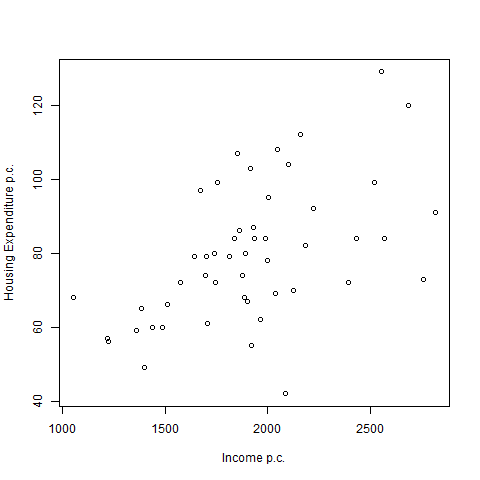
\includegraphics[width=1\textwidth]{Y_X1.png}
\end{figure}

\begin{figure}[h!]\centering
	\caption{\footnotesize The relation between Y and X2.}
	\label{fig:plot_2}
	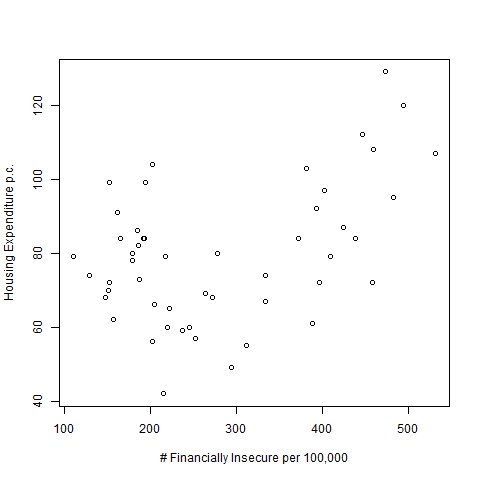
\includegraphics[width=1\textwidth]{Y_X2.png}
\end{figure}

\begin{figure}[h!]\centering
	\caption{\footnotesize The relation between Y and X3.}
	\label{fig:plot_3}
	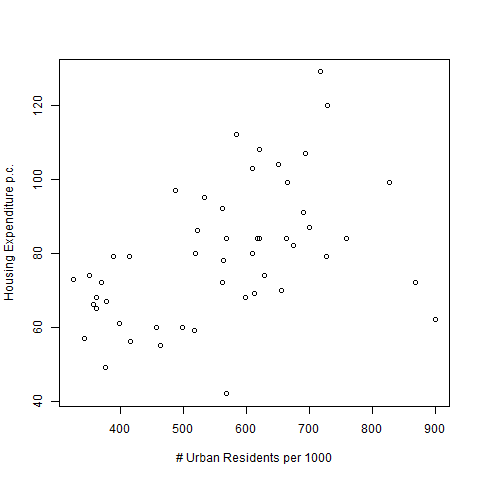
\includegraphics[width=1\textwidth]{Y_X3.png}
\end{figure}

\begin{figure}[h!]\centering
	\caption{\footnotesize The relation between X1 and X2.}
	\label{fig:plot_4}
	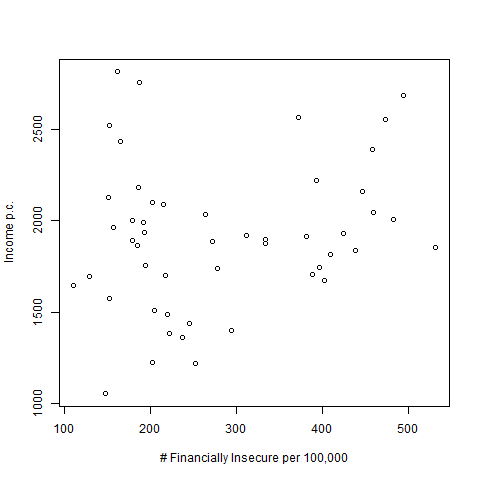
\includegraphics[width=1\textwidth]{X1_X2.png}
\end{figure}

\begin{figure}[h!]\centering
	\caption{\footnotesize The relation between X1 and X3.}
	\label{fig:plot_5}
	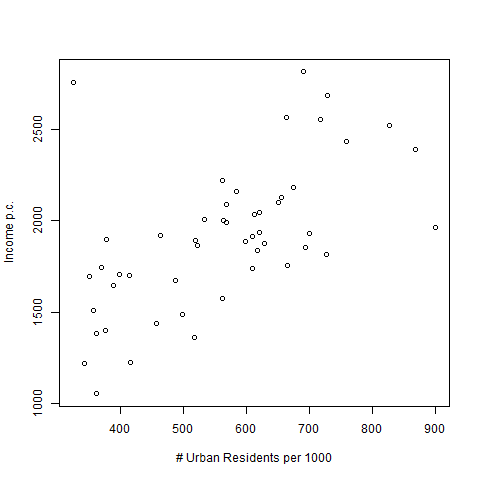
\includegraphics[width=1\textwidth]{X1_X3.png}
\end{figure}

\begin{figure}[h!]\centering
	\caption{\footnotesize The relation between X2 and X3.}
	\label{fig:plot_6}
	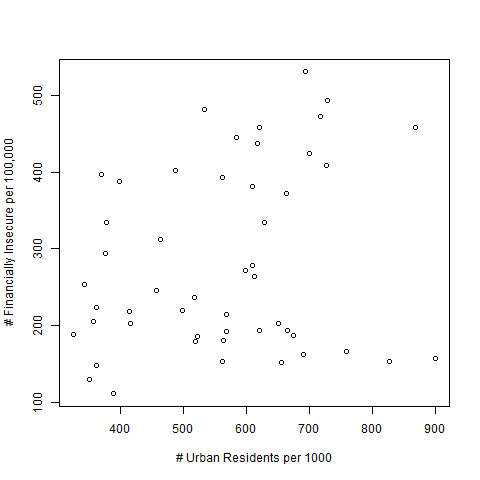
\includegraphics[width=1\textwidth]{X2_X3.png}
\end{figure}

\begin{figure}[h!]\centering
	\caption{\footnotesize Expenditure by Region}
	\label{fig:plot_7}
	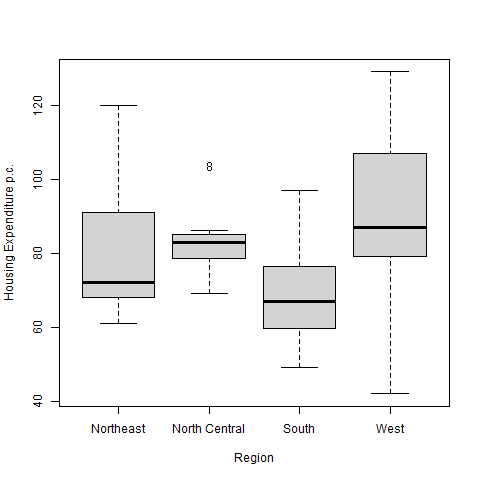
\includegraphics[width=1\textwidth]{Y_Region.png}
\end{figure}

\begin{figure}[h!]\centering
	\caption{\footnotesize The relation between Y and X1, inclusive of Region.}
	\label{fig:plot_8}
	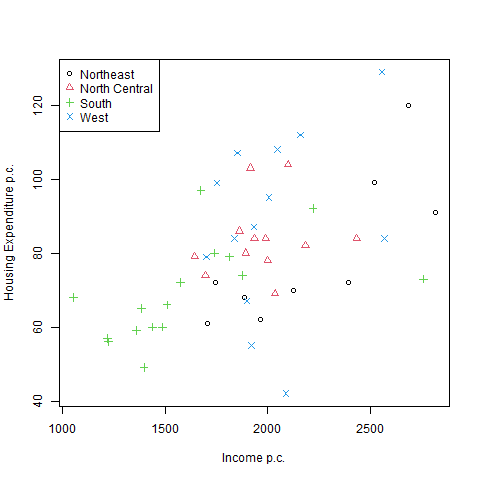
\includegraphics[width=1\textwidth]{Y_X1_Region.png}
\end{figure}

\end{document}
